%-----------------------------------------------------------------------

 \begin{frame}[fragile] 

% The main thing that Enzo struggles with is keeping up with
% the continual exponential increase in parallelism in HPC
% systems.  20 years ago when Enzo was first conceived,
% typical ``massively parallel'' machines had on the order
% of 100 processors, but today's machines have thousands times
% more cores.

% The physics is relatively untouched.  We still want to solve the
% same equations we did 20 years ago.  The numerical methods are also
% mostly the same--hydrodynamics/chemistry are local, FFT's and
% multigrid require some changes but still viable.  The main effect is
% on Enzo's parallel AMR data structures.  AMR meta data didn't used
% to be a problem, but it's a hard limit on scalability now.
% Hierarchy overhead wasn't a problem when it had to loop over
% hundreds of grids, but now it is when it has to loop over millions.
% As hardware parallelism increases, Enzo runs into bottleneck after
% bottleneck, in both memory usage and parallel computation.  Even MPI
% as used in Enzo has limits---barriers and other global operations
% become increasingly costly as core counts increase

% This is what motivated me to start working on Enzo-P/Cello.
% The idea was to redesign and implement the AMR data structure
% from scratch to be as scalable as possible, targeting machines
% that didn't even exist when the project started.  This AMR
% data structure is in a separate reusable framework called Cello.
% Enzo-P is the port of Enzo's physics and numerical methods onto
% Cello.

%---------
% SLIDE 2
%---------

% That's a summary of Enzo's strengths.  Enzo has limitations as well,
% and they are primarily due to the vast increase in size and
% complexity of the high performance computer hardware we have access
% to.  Development on Enzo began about 20 years ago, when ``massively parallel''
% meant about 100 processors.  Today, supercomputers can contain
% a hundred *thousand* processors.  This has affected the three conceptual layers of 
% Enzo in different ways.

% [PHYSICS] The higher-level mathematical equations defining the physics
% are mostly unchanged.  The equations for hydrodynamics and gravity are the
% same today as they were 20 years ago.  Enzo has certainly increased
% its range of problems it can solve, for example by adding support for MHD and RHD,
% but the existing physics requirements are unchanged.

% [METHODS] Numerical methods in Enzo are still very usable for the
% most part.  Methods for solving localized physics such as
% hydrodynamics and chemistry and cooling have the same requirements
% as 20 years ago, and those for global physics such as self-gravity
% are based on FFT's and multigrid, which are still usable on todays
% supercomputers, though may require some optimizations in terms of
% structuring the data

% [DATA STRUCTURES] Which brings us to data structures.  Of these
% three, supercomputer growth has affected the usability of Enzo's
% data structures the most.  Unfortunately, they're also the most
% difficult to change, since all of Enzo's numerical methods use them,
% and changing any part of how Enzo does AMR can lead to a global
% effect on the code.

% [ENZO-P] This is why several years ago I started working on Enzo-P
% and Cello.  Enzo-P serves to contain the physics capabilities and
% numerical methods in Enzo, whereas Cello serves to implement a
% totally new AMR framework designed to be highly scalable, capable of
% running on petascale and ultimately exascale machines.  Needless to
% say, designing software to run on classes of machines that don't
% exist yet is difficult, though a lot of thought has been put into
% making Cello as scalable as possible, so that Enzo's physics can
% continue to live and thrive for many years to come.

\secframetitle{\ssMotivation}
%  \framesubtitle{\enzo's struggles}
 \centerline{\textbf{ENZO has difficulties scaling to modern HPC platforms}} \ \\
 \begin{minipage}{3in}
\pause
  \begin{itemize}
   \item Ever-changing software requirements
     \begin{itemize}
\footnotesize
   \item  Enzo was born in early 1990's
   \item ``massive parallelism'' meant $P\approx 100$
   \item $\times 10^5$ parallelism today
     \end{itemize}
   
\pause
   \item Affects different parts of \enzo\ differently
     \begin{itemize}
   \item[\smiley] \textcolor{red!80!black}{physics} requirements unchanged
   \item[\smiley] \textcolor{green!50!black}{numerical methods} mostly viable
   \item[\frownie] \textcolor{blue}{\textit{data structures}} limit Enzo's scalability
     \end{itemize}
\pause
   \item Motivates AMR data structure redesign
   \begin{itemize}
   \footnotesize
   \item  \textbf{\enzop}: ``petascale'' version of \enzo
   \item keep \enzo's \textcolor{red!80!black}{physics} and many \textcolor{green!50!black}{methods}
   \item  built on \textbf{\cello} \textcolor{blue}{scalable AMR framework}
   \end{itemize}
  \end{itemize}
\end{minipage}
\begin{minipage}{1in}
   \footnotesize
    \centerline{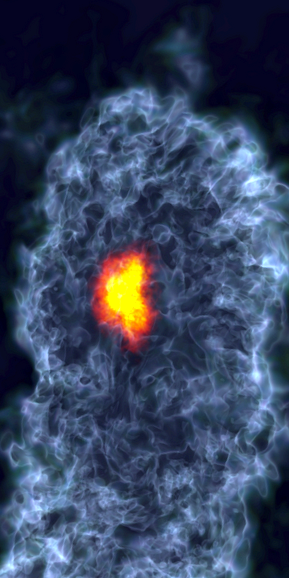
\includegraphics[width=0.875in]{PopIII_vr-edit.png}}
    \centerline{\tiny {[ Sam Skillman, Matt Turk ]}}
\end{minipage}
\end{frame}
